% UTF-8 encoding
% Compile with latex+dvipdfmx, pdflatex, xelatex or lualatex

\documentclass[hyperref, UTF8]{ctexart}
\usepackage{graphicx}
\usepackage{amssymb}
\usepackage{amsmath}
\usepackage{subfigure}
\usepackage{geometry}
\usepackage{caption}
\usepackage{upgreek}
\newcommand{\volt}{{\rm V}}
\newcommand{\source}{{\rm S}}
\newcommand{\ampere}{{\rm A}}
\newcommand{\milliampere}{{\rm mA}}
\newcommand{\hertz}{{\rm Hz}}
\newcommand{\kilohertz}{{\rm kHz}}
\newcommand{\megahertz}{{\rm MHz}}
\newcommand{\ohm}{\Omega}
\newcommand{\kiloohm}{{\rm k}\Omega}
\newcommand{\watt}{{\rm W}}
\newcommand{\kilowatt}{{\rm kW}}
\newcommand{\degree}{^{\circ}}
\newcommand{\farad}{{\rm F}}
\newcommand{\microfarad}{{\rm \upmu F}}
\newcommand{\millifarad}{{\rm mF}}
\newcommand{\henry}{{\rm H}}
\newcommand{\decibel}{{\rm dB}}
\newcommand{\J}{{\rm j}}

\title{电子学基础——第二次仿真作业}
\author{LXQ}
\date{2019.11.22}

\geometry{left=2.0cm, right=2.0cm, top=2.5cm, bottom=2.5cm}
\linespread{1}

\begin{document}

\maketitle

\paragraph{1}
通过仿真画出NMOS和PMOS在不同栅压下的
$I_D-V_{DS}$曲线,并从中取值得出$V_{od}$随着
$V_{GS}$的变化关系。

\paragraph{答}

(1) NMOS的仿真电路图如图 1 所示。
\begin{figure}[!htb]
    \centering
    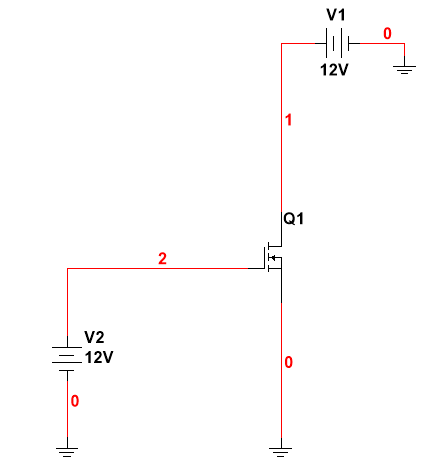
\includegraphics[width=0.291\textwidth]{cir1-1-a.png}
    \caption*{图 1 NMOS仿真电路图}
\end{figure}
其中,在$V_{GS}$分别为$3\volt$和$12\volt$时,所测得的$I_D-V_{DS}$曲线分别如图 2,图 3 所示。

\begin{figure}[!htb]
    \centering
    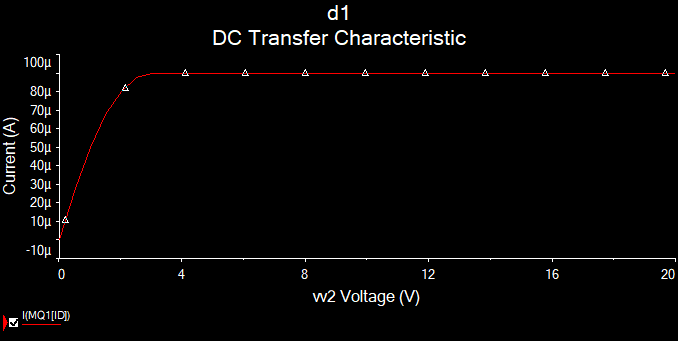
\includegraphics[width=0.452\textwidth]{res1-1-a-2.png}
    \caption*{图 2 $V_{GS}$为$3\volt$时的$I_D-V_{DS}$曲线}
\end{figure}

\begin{figure}[!htb]
    \centering
    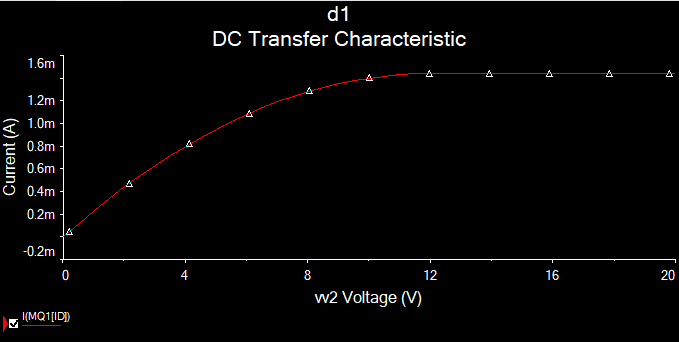
\includegraphics[width=0.453\textwidth]{res1-1-a-1.png}
    \caption*{图 3 $V_{GS}$为$12\volt$时的$I_D-V_{DS}$曲线}
\end{figure}

由饱和区公式在饱和区,两图的电压$I_{D}$分别为$0.09\milliampere$和$1.44\milliampere$,即相差$16$倍。
而两者$V_{GS}$分别为$3\volt$和$12\volt$,即相差$4$倍。由$I_D$与$V_{od}$成平方比,可知$V_{GS}$和
$V_{od}$成正比关系。

(2) PMOS的仿真电路图如图 4 所示。
\begin{figure}[!htb]
    \centering
    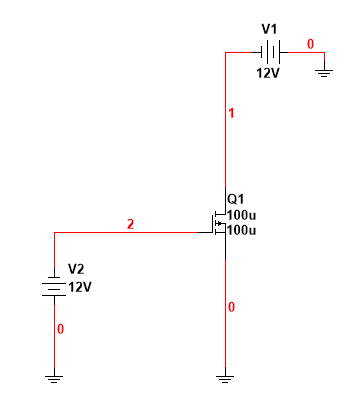
\includegraphics[width=0.236\textwidth]{cir1-2.png}
    \caption*{图 4 PMOS仿真电路图}
\end{figure}
其中,在$V_{GS}$分别为$-3\volt$和$-12\volt$时,所测得的$I_D-V_{DS}$曲线分别如图 5,图 6 所示。

\begin{figure}[!htb]
    \centering
    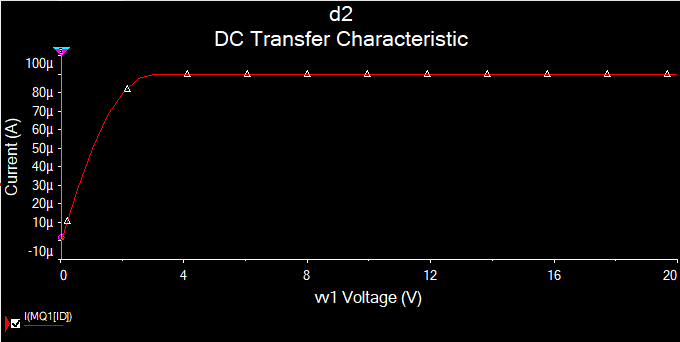
\includegraphics[width=0.453\textwidth]{res1-2-1.png}
    \caption*{图 5 $V_{GS}$为$-3\volt$时的$I_D-V_{DS}$曲线}
    \end{figure}

\begin{figure}[!htb]
    \centering
    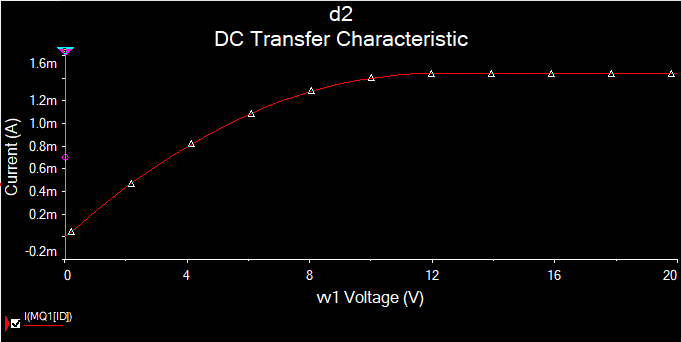
\includegraphics[width=0.454\textwidth]{res1-2-2.png}
    \caption*{图 6 $V_{GS}$为$-12\volt$时的$I_D-V_{DS}$曲线}
\end{figure}
同上分析,仅$V_{GS}$符号改变,则$-V_{GS}$和$V_{od}$成正比关系。

\newpage 

\paragraph{2}
简单设计两个基本共源放大器,一个是电阻负载,一个是二极管
接法的MOSFET负载。并讨论随着输入交流小信号频率的增加,
增益的变化。当频率达到何值时,增益比低频时下降$3\decibel$?

\paragraph{答}
此前曾经用同上一题中的MOS管但是产生的幅频曲线无论如何增加频率,增益都没有下降。因而参考老师
提供的仿真文件使用了如下图 7 中所示的MOS元件。两电路图如图 7 所示。
\begin{figure}[!htb]
    \centering
    \begin{minipage}[t]{0.354\textwidth}
    \centering
    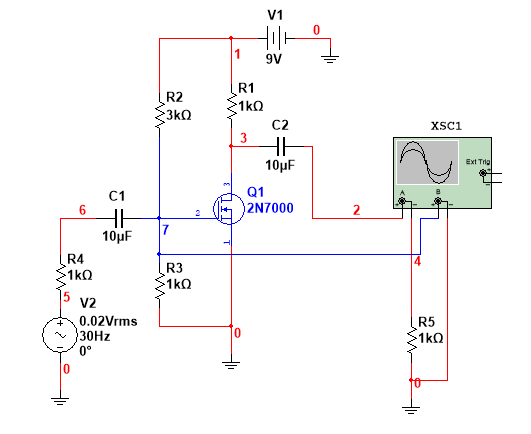
\includegraphics[width=1\textwidth]{cir2-a.png}
    \caption*{(a) 电阻负载}
    \end{minipage}
    \begin{minipage}[t]{0.349\textwidth}
    \centering
    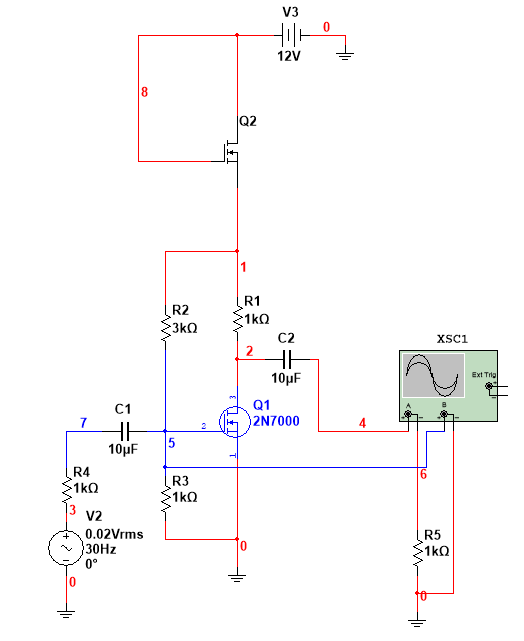
\includegraphics[width=1\textwidth]{cir2-b.png}
    \caption*{(b) 二极管接法}
    \end{minipage}
    \caption*{图 7 共源放大器仿真电路图}
\end{figure}

幅频曲线如图 8 所示。图中蓝色、红色、绿色线分别为输入电压、输出电压以及增益。
\begin{figure}[!htb]
    \centering
    \begin{minipage}[t]{0.453\textwidth}
    \centering
    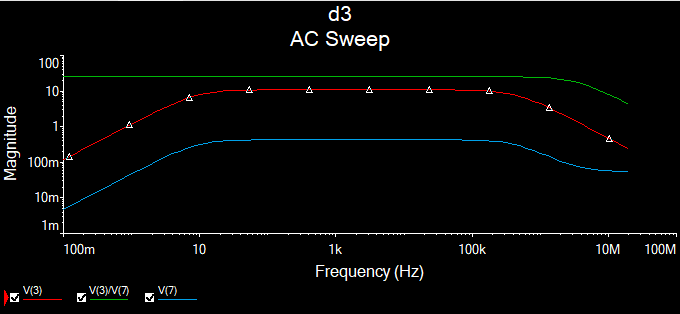
\includegraphics[width=1\textwidth]{res2-a.png}
    \caption*{(a) 电阻负载}
    \end{minipage}
    \begin{minipage}[t]{0.454\textwidth}
    \centering
    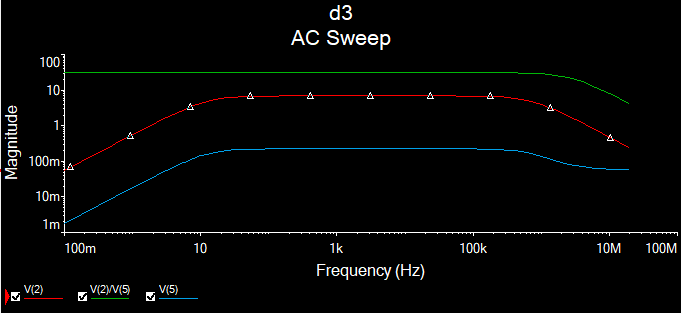
\includegraphics[width=1\textwidth]{res2-b.png}
    \caption*{(b) 二极管接法}
    \end{minipage}
    \caption*{图 8 幅频曲线仿真结果}
\end{figure}

从图中可以看出,无论是电阻负载接法还是二极管接法,在频率较小范围内,电压增益均为定值。
但当频率超过$100\kilohertz$时,电压增益逐渐下降。在电阻负载接法中,频率较小时,增益为
约为$25.0$;当频率增加到$3.4\megahertz$时,增益下降到$17.8$,即下降了$3\decibel$。在二极管
接法中,频率较小时,增益约为$30.6$,当频率增加到$2.7\megahertz$时,增益下降到$21.6$,即下降了
$3\decibel$。

\end{document} 